This chapter is based on work in collaboration with David W. Hogg, Shy Genel, and Soledad Villar.

\graphicspath{{figures/figures_eqcosmo/}}


\section{Chapter Abstract}
The laws of physics obey exact symmetry properties.
The method of invariant scalars is a lightweight and physically motivated way to encode these symmetries in analysis methods, by compressing inputs into scalars that are invariant to rotations, translations, and permutations (particle labeling).
We apply this approach to analyze the relationship between dark matter (DM) and baryons in cosmological simulations, which is critical for understanding the galaxy--halo connection and inferring cosmological parameters from large-scale structure.
Using IllustrisTNG simulation data, we build a training set consisting of DM halos in the DM-only simulation and their corresponding central galaxies in the matched hydrodynamical simulation. 
For each DM halo, we construct a large set of invariant scalars based on geometric phase-space properties of the DM particle distribution.
With these scalars as inputs, we use a neural network to predict the properties of the corresponding galaxies, most importantly the stellar mass.
We show that our approach outperforms the use of standard halo summary properties as the features, as well as using the same geometric information but not compressed into invariant quantities.
The exact symmetries inherent to our method impose informative constraints while preserving the known invariance properties of large-scale structure.
Further, our results are interpretable in terms of the information in DM phase-space and give insight into the connection between galaxy and DM halo properties, relevant to open questions in galaxy formation including the importance of assembly bias on the galaxy--halo connection.


\section{Introduction}

Overdense regions of dark matter (DM) in the universe collapse to form DM ``halos'', which merge and grow to form the underlying structure of the cosmic web (e.g. \citealt{davis_evolution_1985,bond_how_1996,boylan-kolchin_resolving_2009}). 
These DM halos play host to the galaxies that populate our universe, and DM evolution and galaxy formation are deeply intertwined. 
The merger history of halos affects how their galaxies develop, and galactic feedback can in turn affect the growth of structure.
This relationship, known as the galaxy--halo connection \citep{WechslerTinker2018}, is core to both galaxy formation and large-scale structure.

Cosmological hydrodynamic simulations have become extremely powerful tools to model the formation of structure and galaxies (e.g. \citealt{springel_gadget_2001, genel_introducing_2014,dave_simba_2019}).
However, they are very computationally expensive, consuming millions of CPU-hours; even their DM-only counterparts are relatively expensive.
Recently, there have been efforts to \emph{emulate} these cosmological simulations with faster tools, such as machine learning (ML) techniques.
These offer the opportunity to both help us understand the key physical processes affecting structure galaxy formation, as well as construct the large number of mock galaxy catalogs needed to analyze current galaxy surveys. 

There is a growing body of work on learning the relationship between dark matter and galaxy properties using ML-based approaches.
Many of these use a small set of properties of identified DM halos as input features, and focus on predicting the galaxy stellar mass as well as other baryonic properties.
\cite{jo_machine-assisted_2019} show that using extremely randomized trees (ERTs) and including a two-stage learning approach and environmental property features produce accurate galaxy property predictions in the IllustrisTNG simulation.
\cite{lovell_machine_2021} use ERTs to learn the relationship between halos in the EAGLE simulation and galaxies in the zoom C-EAGLE simulations of galaxy clusters.
\cite{de_santi_mimicking_2021} compare the performance of different ML models on predicting galaxy properties from IllustrisTNG, and find success in predicting the stellar mass and reproducing galaxy power spectra.
\cite{delgado_modeling_2021} use a random forest regressor to identify key secondary halo properties for modelling the galaxy--halo connection using IllustrisTNG.
\cite{stiskalek_scatter_2022} also explore how secondary halo properties affect the galaxy--halo connection, specifically analyzing the scatter in the stellar-to-halo mass relation in IllustrisTNG using a neural network ensemble.   
\cite{jespersen_learning_2022} use graph neural networks on DM halo merger trees of halos in the DM-only IllustrisTNG simulation to predict galaxy properties computed from semi-analytic models.

Other works use the dark matter density field as inputs, rather than halo features.
This approach operates on inputs closer to the raw data, but presents its own challenges such as the high sparsity in the stellar mass distribution.
\cite{yip_dark_2019} implement a cascade of convolutional neural networks (CNNs) to predict the 3D galaxy distribution from a voxelization of the IllustrisTNG DM-only simulation.
Along a similar vein, \cite{kasmanoff_dm2gal_2020} predict the stellar mass in voxels centered on subhalos using CNNs in IllustrisTNG.

Another line of inquiry seeks to use ML to emulate and understand structure formation in the dark sector.
Many works have explored using neural networks to map the initial displacement field of a particle grid as to the final displacement field, targeting a full or approximate N-body simulation \citep{he_learning_2018,jamieson_field_2022}.
Others aim to map the final displacements from a very inexpensive N-body simulation substitute to a more realistic output \citep{piras_fast_2023}. 
To develop a deeper understanding of structure formation, \cite{lucie-smith_insights_2022} use gradient-boosted trees to predict late-time mass profiles of DM halos based on input initial conditions and elucidate the relevant scales at play.
\cite{etezad-razavi_unravelling_2023} investigate the role of the velocity field on DM halo masses using CNNs.

While ML techniques are extremely powerful at making predictions, they are generally agnostic to the underlying physical processes they model.
One key aspect of physical laws is \emph{symmetries}: we expect that our results will change in exact ways, or not change at all, under certain transformations.
Some ML models are naturally \emph{equivariant} to certain symmetries, such as convolutional neural networks to translations and graph neural networks to permutations.
Recently, additional ML approaches that enforce physical symmetries have been developed.
CNNs have been extended to incorporate rotational symmetries \citep{cohen2019gauge,wang2021incorporating,ocampo_scalable_2023}.
Most relevant to our focus on simulated dark matter halos,neural networks that operate on point clouds have been developed that enforce rotation, translation, and permutation equivariance using a variety of approaches.
These include irreducible representations \citep{thomas2018tensor}, self-attention mechanisms \citep{fuchs2020se}, and convolutions \citep{kondor2018covariant,zhang2019rotation}, as well as extensions of graph neural networks \cite{Satorras2021}.

Approaches to learning the galaxy--halo connection that are based on a set of halo properties are often naturally obey obey the relevant symmetries; for instance, mass and concentration are invariant to rotations, translations, and permutations of the DM halo particles.
On the other hand, ML models operating directly on the dark matter density field do not typically respect all of these symmetries.
Recent work has applied explicitly equivariant neural network architectures and approaches to structure formation and the galaxy--halo connection in cosmological simulations.
\cite{dai_learning_2020} use Lagrangian Deep Learning to reproduce both dark matter evolution and hydrodynamical outputs, based on an initial linear density field; this approach respects translational and rotational symmetries.
\cite{thiele_predicting_2022} use permutation- and rotation-invariant DeepSets to predict the thermal Sunyaev-Zel'dovich field in galaxy clusters in IllustrisTNG.

In this work, we propose an equivariant approach to characterizing the dark matter distribution that enforces the known symmetries of cosmological simulations. 
We use the method of \emph{invariant scalars} introduced by \cite{Villar2021a}, which offers a lightweight approach to representing invariant and equivariant functions using a collection of scalar quantities.
The core idea is that geometric objects---such as vectors of particle positions and velocities---can be \emph{contracted} to form scalars that are invariant to transformations, namely translations, rotations, velocity boosts, and permutations.

Recent work has shown that this ``scalars'' approach improves performance on prediction tasks.
\cite{yao_simple_2021} demonstrated the approach on a toy dynamical system and showed that it outperformed state-of-the-art approaches in both speed and accuracy.
It has recently been applied to large-scale structure problems: \cite{villanueva-domingo_learning_2022} used scalars in combination with graph neural networks applied to simulated galaxy catalogs to perform cosmological inference.
\cite{thiele_predicting_2022} constructed invariant scalars from input dark matter particles as well as galaxy cluster-scale features as inputs to their DeepSet architecture.

We apply the invariant scalars approach to the particle distribution of DM halos in the IllustrisTNG DM-only simulation.
To obtain a uniform set of features across halos while preserving detailed structure, we first compress the DM halo particles into geometric multipole moments in radial bins, and then combine these into invariant scalar features.
This provides a characterization of DM halos that encodes interpretable, high-order phase-space structure while preserving physical symmetries.
To learn the mapping from DM halos to baryonic properties, we construct a set of matched DM halos in the DM-only simulation to central galaxies in the TNG hydrodynamical simulation.
We use a XXX model with the scalars as inputs to predict galaxy properties, and compare this approach to benchmark feature sets. 
We also demonstrate that these features allow for accurate predictions of the mass assembly history of the DM halos.

In this work, we use the following notation: 
Scalars are denoted by lowercase variables, vectors by lowercase bold variables, and tensors by uppercase variables.

This paper is outlined as follows.
In \S\ref{sec:sim_sample}, we introduce the simulation used and our halo and galaxy sample selection. 
We discuss our approach to constructing invariant scalars from dark matter halo particle distributions in \S\ref{sec:scalars_approach} 
In \S\ref{sec:features_model}, we detail the fiducial scalar feature set and other benchmark feature sets we use as inputs, and describe the prediction model.
In \S\ref{sec:results}, we present the results of predicting the mass assembly history and galaxy properties from DM halo features, and in \S\ref{sec:discussion}, we interpret these results and discuss their implications and applications.
We summarize our results and conclusions in \S\ref{sec:summary}.


\section{Simulation and Sample Construction}
\label{sec:sim_sample}

\subsection{The IllustrisTNG simulations}
\label{sec:sim}

The Illustris TNG simulations are cosmological magnetohydrodynamical simulations that co-evolve dark matter and baryons to model galaxy formation \citep{springel_first_2018,nelson_first_2018,pillepich_first_2018,naiman_first_2018,marinacci_first_2018}.\footnote{Data products from the TNG Project are publicly accessible at \url{https://www.tng-project.org/}.}
The simulations are run starting from initial conditions at $z=127$ with cosmological parameters from \cite{ade_planck_2016} $\Omega_m = \Omega_{dm} + \Omega_b = 0.3089$, $\Omega_b = 0.0486$, $\Omega_\Lambda = 0.6911$, Hubble constant $H_0 = 100$ $h$ km s$\inv$ Mpc$\inv$ with $h = 0.6774$, $\sigma_8 = 0.8159$, and $n_s = 0.9667$.
They model baryonic processes including ionizing background radiation, star formation and stellar feedback, stellar evolution and chemical enrichment, pressurization of the interstellar medium from supernovae, and the growth of and feedback from supermassive black holes.   
We use the TNG-100-1 simulation, which has a size of $L = (75 \hMpc)^3$, $1820^3$ DM particles and the same number of gas cells, and mass resolutions of $m_\text{DM} = 7.5 \times 10^6 \Msun$ and $m_\text{gas} = 1.4 \times 10^6 \Msun$.
The simuluation also evolves star/wind and black hole particles.
It has a matched DM-only simulation run with the same initial conditions, TNG-100-1-Dark, with mass resolution of $8.9 \times 10^6 \Msun$.
We refer to the DM-only simulation (TNG100-1-Dark) as \dark and the hydrodynamical simulation (TNG100-1) as \hydro in the rest of this work.
For most of this work, unless otherwise stated, we use the $z=0$ snapshot.

We use the DM halo catalogs provided by the TNG project as the starting point for our sample.
Halos are defined by a Friends-of-Friends (FoF) algorithm on DM particles, with a linking length of 0.2 times the mean inter-particle separation; other types of particles are assigned to the same halo as their nearest DM particle.
Subhalos within halos are found using the Subfind algorithm, which identifies gravitationally bound structures across all particle types.


\subsection{Halo and galaxy sample selection}
\label{sec:select}

One of our goals with this project is to propose a characterization of DM halos that is useful for predicting the properties of the galaxies they host, as well as their assembly history.
Given this, we operate on the halos in the \dark (DM-only) simulations, with the idea of learning the results of the hydrodynamic galaxy formation model.
To that end, we construct a sample of paired DM halos in the \dark simulation and galaxies in the \hydro (full hydrodynamical) simulation. 
We consider only central galaxies in this work; the approach could be straightforwardly extended to satellite galaxies.

We first make a cut on the \dark halos, choosing only halos with a mass $\Mfof > 10^{10.25} \, \hMsun$, where $\Mfof$ is the mass of all the particles that are part of the FoF group within $\Rtwoh$, and $\Rtwoh$ is the radius enclosing a mass of 200 times the mean density of the simulation.
We use this mass definition, as opposed to the typical $\Mtwoh$ which includes all particles both part of and not part of the FoF group, as our approach will operate only on the FoF particles and this keeps the mass definitons consistent; however, this is just for technical reasons, and only differs at the few percent level.
We require that the halos have at least one subhalo.
We use the matched subhalo catalogs provided by the TNG Project, which match subhalos in the dark simulation to subhalos in the paired hydrodynamical simulation; we call these subhalo pairs ``twins''.
The matching is done with the ``LHaloTree'' algorithm, which selects the halo in the other simulation with the largest number of DM particles in common, and requires that both simulations agree, resulting in bijective matches.
We discard halos that do not have a \hydro match.
For every \dark halo, we take its most massive \dark subhalo.
For that \dark subhalo, we find its twin \hydro subhalo.
We consider the baryons in this subhalo to constitute the central galaxy that is associated with the original \dark halo; we call this the ``matched'' galaxy of the \dark halo. 
We note that this twin \hydro subhalo is nearly always (but occasionally not) the most massive subhalo in its parent halo in the \hydro simulation.

We make some additional cuts on this sample.
We note that some of these cuts are on the ``labels'' or otherwise require knowledge of the hydrodynamical simulation; in a full application this should be handled more carefully, such as implementing an additional prediction step. 
We discard all \dark halos for which the twin \hydro subhalo has fewer than 50 star particles.
We discard all pairs for which the mass $\Mtwoh$ of the DM halo and the matched hydro halo differ by a factor of 3 or more; we assume that this indicates a bad match, and only occurs for a very small fraction of halos.
We also require that the SC-SAM has been applied to the halos, as we use the halo assembly histories computed by the SC-SAM (discussed further in \S\ref{sec:mah}); this removes a few percent of the halos.
These selections result in XXX \dark halos and matched \hydro galaxies.
We use 70\% as a training set, 15\% as a validation set, and 15\% as a test set.


\subsection{Halo mass assembly history}
\label{sec:mah}

We aim to predict the mass assembly history of the \dark halos based only on their present-day ($z=0$) properties.
This is informative as it captures the dynamical history of the halo, which affects the formation of the galaxies it hosts.
We use the merger histories computed by \citep{gabrielpillai_galaxy_2021} as part of a comparative analysis between TNG and the Santa Cruz semi-analytic model (SC-SAM, \citealt{somerville_semi-analytic_1999,somerville_semi-analytic_2008, somerville_star_2015}); the SAM is based on these merger trees.\footnote{The merger history and other SC-SAM data is publicly accessible at \url{https://github.com/aust427/illustris_sam}.}
The merger trees are run on halos found with the \textsc{rockstar} \citep{behroozi_rockstar_2013} code and built with \textsc{consistent trees} \citep{behroozi_gravitationally_2012}, and a bijective matching is performed between the \textsc{rockstar} and TNG Subfind halos.

We consider the most massive progenitor branch of the assembly history of each \dark halo in our sample.
We compile the mass of the halo's most massive progenitor for each of the TNG snapshots. 
A natural quantity to try to predict would be the fraction of the $z=0$ halo mass accreted as a function of redshift.
However, different halos can be traced back to different redshifts, and this inconsistency causes difficulties at the prediction stage.
We thus choose to learn the scale factor $a$ (related to the redshift $z$ by $a=1/(1+z)$) at which the halo has accreted a given fraction of its mass, $M_\mathrm{vir}(a)$/$M_\mathrm{vir}(a=1)$, where $M_\mathrm{vir}$ is given by the \field{HalopropMvir} field of the SC-SAM data and $a=1$ is the present day.
This swapped quantity gets at the same information as the natural quantity but is more stable in predictions.
We compute this at XXX linearly spaced mass fractions between 0 and 1 (exclusive). 
As we only have the history at a finite number of snapshots, we perform a linear interpolation between the mass fractions and scale factors to estimate the scale factor at a given mass fraction.
If the target mass fraction is outside the bounds of the data (for example, if the initial mass of the halo was a larger mass fraction than our tabulated values), we assign the scale factor to be that at which the mass fraction is closest.  



\subsection{Galaxy properties}
\label{sec:galprops}

% TODO: add uncertainty info here
We aim to predict the properties of central galaxies hosted by a given dark matter halo.
In this section we detail these properties and the associated choices we make. 
We choose to predict only scalar properties for this work, as we focus on enforcing \emph{invariance} to physical symmetries, though we could also predict vector and higher order properties and enforce \emph{equivaraince}.

The primary target is the galaxy stellar mass $\mstellar$, the mass of all of the star particles belonging to the twin \hydro subhalo of the \dark halo.
We use the TNG field \field{SubhaloMassType} for star particles, and convert to units of log($\hMsun$).
Stellar mass is the main quantity used for creating mock catalogs, and is tightly coupled to nearly all other galaxy properties, so we focus on this quantity in this work.
We also aim to predict the following other baryonic properties: 
the stellar half-mass radius $\rstellar$, the specific star formation rate averaged over 1 Gyr $\ssfr$, the specific stellar angular momentum $\jstellar$, the black hole mass $\mbh$, and the color $\gminusi$. 
The stellar radius $\rstellar$ is the TNG property \field{SubhaloHalfmassRadType} of the subhalo for star particles, in units of log(kpc/$h$).
The value of $\ssfr$ is based on the star formation rate catalogs provided by the TNG Project \citep{donnari_star-formation_2019,pillepich_first_2019}.
We use the \field{SFR\_MsunPerYrs\_in\_all\_1000Myrs} field, the star formation rate including all bound star particles of the subahlo, and take the ratio with the stellar mass $\mstellar$; we use units of log(yr$\inv$).
For the galaxies that have $\ssfr=0$, we assign a small value based on the average gas mass cell and the 1 Gyr timescale ($\text{SFR}_\mathrm{zero} = 10^{-3} \hMsun \text{yr}\inv$).
We use the $\jstellar$ computed by the approach of \cite{genel_galactic_2015} in the same way as the \field{SpecificAngMom} field in the TNG Project catalog, with units km s$\inv$ kpc. 
The $\mbh$ value is that given by the TNG field \field{SubhaloBHMass} of the subhalo, in units of log($\hMsun$).
For galaxies with zero black hole mass, we assign the value to be half of the minimum black hole mass in our sample. 
We use the $g-i$ color comptuted from synthetic SDSS photometry as provided by the TNG project \citep{nelson_first_2018}; the photometry is in units of AB magnitudes. 
The distributions of these properties as a function of \dark halo mass are shown in the left column of Figure~\ref{fig:galprops}.


\section{The invariant scalars approach}
\label{sec:scalars_approach}

Our method for characterizing DM halos is based on the ``scalars'' approach of \cite{Villar2021a}.
The core idea is that functions invariant or equivariant to certain transformations can be expressed in terms of a set of scalars, constructed from the input quantities.  
This is motivated by the fact that the physical laws that govern the evolution of the universe---and thus cosmological simulations---obey exact classical symmetries.
We outline our approach here to apply the scalars approach to DM halo characterization and prediction tasks, and go into further detail in the rest of this section.

Our goal is to characterize DM halos in a way that captures detailed phase-space structure while enforcing invariance to transformations.
(The same approach applies to equivariance, but here we aim to predict scalar properties and thus focus on invariance.)
We specifically consider rotation, translation, velocity boosts, rotation, and permutation (of the particles); these are detailed in \S\ref{sec:symmetries}.
For each \dark halo, we use a multipole expansion to compress the particle positions and velocities of each halo into a set of ``geometric features'' that describe the phase-space structure of the halo; this is discussed in \S\ref{sec:geometric_features}.
We then construct scalar contractions of these geometric features, which are scalars, vectors, and tensors; these ``scalar features'' are invariant to transformations of the particles. 
This step is informed by Einstein summation notation, which only allows invariant scalars to be produced; the details of our scalar feature construction is discussed in \S\ref{sec:scalar_features}.
We can finally use these scalar features as the inputs for our prediction task; in our case we use a Gradient Boosted Tree model (\S\ref{sec:prediction_model}), though we note that the scalars could be used with other model choices.

In contrast to this approach, many standard approaches use a small set of hand-constructed properties of the halos, such as the mass, concentration, and spin.
While these do often obey physical symmetries, this is not enforced; further, the properties are hand-picked and can be non-trivial to compute, and they do not necessarily capture the complexity of the phase-space structure of the halos.
We use these ``standard features'' as a benchmark, detailed in \S\ref{sec:benchmarks}.
Other approaches work on the full particle distribution, or the smoothed density field; while this captures the detailed halo structure, it does not obey many of the physical symmetries (depending on implementation), and can be very expensive.
The scalars approach captures the benefits of both of these standard approaches: it allows for a flexible, lightweight set of halo features that respects symmetries and provides a more complete representation of DM structure.
\ksf{move this to discussion?}
We also expect the enforced equivariance to make the approach more generalizable, for instance to different resolutions or simulation codes.


\subsection{The physical symmetries}
\label{sec:symmetries}

% to write
%what is a geometric object? scalars, vectors, tensors - defined by their transformation properties under rotation, translation, permutation. properties that ensure that coordinate freedom preserve angular momentum, linear momentum, etc

\subsection{Geometric features}
\label{sec:geometric_features}

\begin{table}
    \caption{The geometric features we construct from the \dark halo particles, following the multipole expansion of \eqt{eq:geo}. The table gives for each feature its name in multipole moment and more readable notation, its order (rank), and its degree in mass, position, and velocity, and its physical interpretation. All of the geometric features have mass degree of 1 as the are constructed as single sums over masses.}
    \label{tab:geos}
    \vspace{0.5em}
    \centering
    \begin{tabular}{|l|l|l|l|l|l|l|}
    \hline
    moment & name & order & $m$ deg. & $\x$ deg. & $\vel$ deg. & physical interpretation \\
    \hline
    $g_{00n}$ & $m_n$ & 0 & 1 & 0 & 0 & mass in $n$th bin \\
    $g_{10n}$ & $\x_n$ & 1 & 1 & 1 & 0 & mass-weighted position of $n$th bin \\
    $g_{01n}$ & $\vel_n$ & 1 & 1 & 0 & 1 & mass-weighted velocity of $n$th bin \\
    $g_{20n}$ & $\Cxx_n$ & 2 & 1 & 2 & 0 & variance tensor of positions in $n$th bin \\
    $g_{11n}$ & $C^{(\x\vel)}_n$ & 2 & 1 & 1 & 1 & covariance of pos. and vels. in $n$th bin \\
    $g_{02n}$ & $\Cvv_n$ & 2 & 1 & 0 & 2 & variance tensor of velocities in $n$th bin \\
    \hline
    \end{tabular}
\end{table}

We first compute a set of \emph{geometric features} from our data from the particle distribution, specifically their masses, positions, and velocities. 
There are multiple reasons we do this.
Theoretically we could compute scalars directly from the particles that consitute the halo; in fact, this would be simpler as these are all scalars and vector inputs.
However, this results in an enormous number of scalars as it would require the inner product of each pair of particles, scaling as the square of the number of particles.
It also would produce a different number of particles for each halo, which is difficult to handle at the prediction stage.
Finally, the ordering of the scalars is not clear and the permutation invariance would be brittle at best.
By first condensing the particles into a uniform set of geometric features, we circumvent all of these issues.
We note that there are many ways to handle this step, and we have chosen one relatively simple option.

We choose the geometric features to be based on a multipole expansion, computing moments of the data in a set of radial shells. 
We define the geometric features $g_{\ell p n}$ as: 
\label{eq:geo}
\begin{equation}
    g_{\ell p n} = \sum_i m_i \, W_n(r_i) \, \left( \x_i^{\otimes \ell} \, \otimes \, \vel_i^{\otimes p} \right)
\end{equation}
where $i$ indexes the particle, $m_i$ is the mass of the $i$th particle, $W_n(r_i)$ is the $n$th window function (defining the radial bins), and $r_i$ is the distance between the position of the $i$th particle and some fiducial point.
% TODO: should switch this position thing in code to be clear, then update here
We choose this fiducial point, which functions as the halo center, to be the location of the most bound particle in the halo (the particle with the minimum potential energy), as given by the TNG field \field{SubhaloPos} for the halo's central subhalo (for our sample, this is equivalent to \field{GroupPos} of the \dark halo).
The quantity $x_i^{\otimes \ell}$ is the $\ell$th moment (outer product $\ell$ times) of the particle position (with respect to the fiducial point).
For $\ell = 0$, this is 1; for $\ell = 1$, this is the vector position of the particle; and for $\ell = 2$, this is a tensor computed from the outer product of the particle position with itself; and so on.
The quantity $v_i^{\otimes p}$ is the same but for the velocities, with $p$ indexing the velocity moments, where the velocities are with respect to the center of mass velocity of all the particles in the halo.

The geometric features up to second order in $\ell + p$ are shown in Table~\ref{tab:geos}.
They all have the same mass order, $O(m)=1$, as they just include a sum over particle masses.
The $\x$ and $\vel$ orders are determined by the $\ell$ and $p$ values.
We see that $g_{00n}$ are scalars, $g_{01n}$ and $g_{10n}$ are vectors, $g_{20n}$, $g_{02n}$, and $g_{11n}$ are (rank-2) tensors, and so on.
These geometric features have, at least at low order, interpretable meaning in terms of the halo shape; we give them names based on this.
In the $n$th window, $g_{00n}$ ($m_n$) is the mass of all the particles in that bin; $g_{10n}$ ($\x_n$) is their mass-weighted position (note that it is not quite the center of mass position because we do not divide out the total bin mass); $g_{01n}$ ($\vel_n$) is their mass-weighted velocity; $g_{20n}$ ($\Cxx_n$) is the variance tensor of the positions; $g_{02n}$ ($\Cvv_n$) is the variance tensor of the velocities; and $g_{11n}$ ($C^{(\x\vel)}_n$) is the covariance tensor of the positions and velocities.
In the rest of this work, we use these names for readability.
\ksf{what notation should i be using for the orders, O()? should also figure out diff bw order and degree!}

We make the following choices when computing our set of geometric features.
We compute the geometric features up to second order in position and velocity combined, $O(\x) + O(\vel) \leq 2$ (as shown in Table~\ref{tab:geos}); this means we don't have objects of higher rank than a rank-2 tensor.
We use a top-hat window function producing hard-edged bins. 
Our bins are functions of halos radius, defined by $\Rtwoh$, the radius that encloses a mass of 200 times the mean density of the universe at that time.
For our fiducial features, we choose three bins within $\Rtwoh$, chosen to represent different regions of the halo: the inner core, the middle region, and the outer halo.
These are defined by bin edges $[0, 0.1\Rtwoh, 0.4\Rtwoh, \Rtwoh]$, and we index them by $n=[0,1,2]$ in our notation.

We rescale the geometric features to make them dimensionless.
We divide out factors of $\Mfof$, $\Rtwoh$, and $\Vfof$ (computed as $\sqrt{G\Mfof/\Rtwoh}$ where $G$ is the gravitational constant) based on the mass, position, and velocity order respectively; for example, for $\x$ we divide out one factor of $\Mfof$ and one of $\Rtwoh$.

We also we must specially handle the features $C^{(\x\vel)}_n$, as the ordering of the $\x$ and $\vel$ terms in the product matters.
In this case, we can construct the symmetric feature $ \CxvS_n = \frac{1}{2} (C^{(\x\vel)}_n + C^{(\vel\x)}_n)$ and the antisymmetric feature $\CxvA_n = \frac{1}{2} (C^{(\x\vel)}_n - C^{(\vel\x)}_n)$.
These are pseudotensors, and thus require special handling when constructing the scalars, detailed in the next section.

This procedure results in 7 geometric features per bin; for our 3 fiducial bins, this is 21 features per halo.

\subsection{Invariant scalar features}
\label{sec:scalar_features}

\begin{figure}
    \centering
    %\includegraphics{}
    \caption{A selection of dark matter halos of fixed mass (M=YYY), colored by the value of one of the invariant shape scalars, XXX. The central galaxy each one hosts is shown in the bottom row, colored by its stellar mass; the invariant scalar is correlated with the stellar mass, demonstrating how it is a useful predictor for the galaxy--halo connection.}
    \label{fig:halo_viz}
\end{figure}


\begin{table}
    \caption{The scalar features constructed from the geometric features, up to second degree in $m$, and up to fourth degree in each of $\x$ and $\vel$. All of the features have order 0 as they are rank-0 scalars. The indices $n$ and $n'$ index the radial bins of the geometric features, $q$ and $q'$ index the eigenvalues, and $j$ and $k$ are the indices summed over in Einstein summation notation. We show the vector notation and/or and Einstein summation notation depending on whether there is a clear representation in that notation.} 
    \label{tab:scalars}
    \vspace{0.5em}
    \centering
    \begin{tabular}{|l|l|l|l|l|l|l|}
    \hline
    vector not. & summation not. & order & $m$ deg. & $\x$ deg. & $\vel$ deg. \\
    \hline
    $m_n$ & $m_n$ & 0 & 1 & 0 & 0 \\
    $\lambda_q(\Cxx_n)$ & & 0 & 1 & 1 & 1 \\
    $\lambda_q(\CxvS_n)$ & & 0 & 1 & 2 & 0 \\
    $\lambda_q(\Cvv_n)$ & & 0 & 1 & 2 & 2 \\
    $\x_n\T \cdot \x_{n'}$ & $[\x_{n}]_j \, [\x_{n'}]_j$ & 0 & 2 & 2 & 0 \\
    $\x_n\T \cdot \vel_{n'}$ & $[\x_{n}]_j \, [\vel_{n'}]_j$ & 0 & 2 & 1 & 1 \\
    $\vel_n\T \cdot \vel_{n'}$ & $[\vel_{n}]_j \, [\vel_{n'}]_j$ & 0 & 2 & 2 & 0 \\
     & $[\Cxx_n]_{jk} \, [\Cxx_{n'}]_{jk}$ & 0 & 2 & 4 & 0 \\
     & $[\Cxx_n]_{jk} \, [\CxvS_{n'}]_{jk}$ & 0 & 2 & 3 & 1 \\
     & $[\CxvS_{n}]_{jk} \, [\CxvS_{n'}]_{jk}$ & 0 & 2 & 2 & 2 \\
     & $[\CxvA_{n}]_{jk} \, [\CxvA_{n'}]_{jk}$ & 0 & 2 & 2 & 2 \\
     & $[\Cxx_{n}]_{jk} \, [\Cvv_{n'}]_{jk}$ & 0 & 2 & 2 & 2 \\
     & $[\CxvS_{n}]_{jk} \, [\Cvv_{n'}]_{jk}$ & 0 & 2 & 1 & 3 \\
     & $[\Cvv_{n}]_{jk} \, [\Cvv_{n'}]_{jk}$ & 0 & 2 & 0 & 4 \\
    \hline
    \end{tabular}
\end{table}

We combine these geometric features with each other to obtain \emph{scalar features}, scalar quantities that are invariant to the desired physical symmetries.
To construct these combinations, we produce all allowed \emph{contractions} of the geometric features that produce scalar quantities.
For instance, one can multiply a pair of scalars; take the inner product of a pair of vectors; take contractions of a pair of tensors; and take the trace or eigenvalues of a tensor.
In fact, when considering up to rank-2 tensors and scalars up to second order in mass, as we do here, these are all of the possible ways of combining geometric features.
(If we considered higher mass orders, we could construct features such as $\x \, \Cxx \, \x\T$.)
One natural way to enumerate these scalars is using Einstein summation notation, as it only allows invariant scalars to be produced (see Appendix~F of \citealt{Villar2021a} for a detailed discussion).
In short, to construct a scalar there must be no hanging indices, so we know that all indices used in the summation must be repeated.

We make some specific choices regarding the computed scalars.
We limit the scalars to second order in $m$, which in our case means a single geometric feature or a combination of two features.
We also limit to fourth order in $\x$ and fourth in $\vel$, though this is already constrained by our second-order limits in these quantities for the geometric feature construction.
We choose to use the eigenvalues $\lambda_q$ of each tensor, where $q=1$ is the maximum eigenvalue and $q=3$ the smallest, as these give more information than just the trace.
We include cross-terms across different bins $n$ and $n'$, and cross-terms between position and velocity geometric features.
For the pseudotensors, namely $\CxvA_n$, we can only contract them with other pseudotensors to construct true scalars (contractions of a pseudotensor with a tensor would result in a pseudoscalar).
The allowed scalar contractions are shown in Table~\ref{tab:scalars}.
With our 3 fiducial bins, this produces 102 unique scalar features.

When we make predictions with these scalar features, we additionally include the mass, radius, and velocity quantities we used to rescale the geometric features: $\Mfof$, $\Rtwoh$, and $\Vfof$. 
This allows us to encode the broad features and the halo shape separately, and understand their relative contributions to prediction tasks.


\section{Feature sets and prediction model}
\label{sec:features_model}

\subsection{Feature sets: scalars and benchmarks}
\label{sec:benchmarks}

Our fiducial feature set is the 102 scalar features per halo described in \S\ref{sec:scalar_features}.
As a baseline comparison for the predictions with our invariant scalar features, we construct other ``benchmark'' feature sets.

The first set is using only the mass, radius, and velocity: $\Mfof$, $\Rtwoh$, and $\Vfof$. 
These quantities are all directly related ($\Mfof$ is the bound mass inside $\Rtwoh$, and $\Vfof$ is proportional to the square root of the ratio of $\Mfof$ and $\Rtwoh$), so this feature set captures broad trends with these basic quantities.

The second is using standard ``catalog'' features that are used in typical approaches to this and related tasks.
We include $\ctwoh$, the halo concentration defined as the dimensionless ratio of $R_{200c}$, the radius enclosing 200 times the critical density of the universe, and $R_\mathrm{s}$, the scale radius computed by fitting an NFW profile to the DM halo density; this is the TNG field \field{c200c} computed by \cite{anbajagane_baryonic_2021}.
We use the one-dimensional velocity dispersion $\sigma_{v}$, computed from the halo's central \dark subhalo, as given by the TNG field \field{SubhaloVelDisp}; this is computed from all particles belonging to the subhalo, and is the 3D velocity dispersion divided by $\sqrt{3}$, in units $km/s$.
We also include the spin $\lambda$, computed as $\lambda = \sqrt{\lambda_x^2 + \lambda_y^2 + \lambda_z^2}$, where the spins along each axis are from the TNG field \field{SubhaloSpin} for the central \dark subhalo, which are the mass-weighted sum of the coordinate along each axis times the relative velocity of all particles.
We additionally include $\Mfof$, $\Rtwoh$, and $\Vfof$ in this set.
Other works include other features such as environmental properties of the local density around the halo, and formation history properties such as the age, formation time, or number of mergers of the halo.
As we only consider $z=0$ features and particles in the halo FoF for our invariant scalars approach in this work, we do not include this environmental and formation properties for a more direct comparison (though this is for simplication purposes and a full analysis for practical use could and should use this information for all feature sets).

We finally consider a set of features constructed from the \emph{components} of the geometric features.
That is, we unroll each geometric feature into its components in $x$, $y$, and $z$, giving 1 quantity for scalars, 3 for vectors, and 9 for tensors, and use these as the feature set. 
Including the components of both the symmetric and antisymmetric components of the position-velocity covariance tensor, this results in 43 features per bin; for our 3 fiducial bin case, this gives 129 features.
We also include the $\Mfof$, $\Rtwoh$, and $\Vfof$ features in this set.


\subsection{Prediction model}
\label{sec:prediction_model}

To predict the desired output scalars, we train a fully collected neural network.

The neural net takes as input a set of scalar features as described in \S\ref{sec:scalar_features} for a given halo, along with the overall quantities used for rescaling, $\Mtot$, $\xrms$, and $\vrms$ (we take their logarithms to reduce the dynamic range).
The labels are the scalar galaxy properties of interest.
The NN consists of XXX layers, with SELU activation functions in between; we choose these because ... 

We use a Gaussian loss function, which takes the form
\begin{equation}
    L = 
\end{equation}
The uncertainties $\sigma$ on the labels are based on the intrinsic scatter as a function of galaxy mass.
We estimate this quantity from the work of \cite{Genel2019}, which quantifies the chaotic behavior of cosmological simulations that leads to random differences in $z=0$ galaxy properties.
The uncertainties used can be found in Figure 8 of that work, for the mass resolution XXX, closest to that of the simulation used in this work.
For galaxies below the mass given in that figure, we ..., and for galaxies above that mass, we use ... \ksf{fill in}.
%Our covariance matrix for our fit $C_\mathrm{data}$ is then a diagonal matrix with the square of these uncertainties along the diagonal.


We split the data into training (70\%), validation (15\%), and test (15\%) sets.
We train the model on the training set for 1000 epochs (passes over the entire training set).
At each pass, we compute the loss over the validation set; we take the final model to be the epoch with the minimum validation loss. 

We perform hyperparameter tuning to determine the optimal learning rate and hidden layer size.
We test a grid of these values: for learning rate, XXX, and for hidden layer size, YYY.
We choose the parameters that have the best precision on the validation set





We also tested a simple linear regression model, but found that it cannot reproduce some of the complexities of the halo--galaxy property distributions.
To alleviate this, we tried inputting known functions as a base and predicting the scatter off of this function, such as the broken power law for the SHMR \citep{}.
This achieved reasonable precision, but was less flexible than the neural net and required more choices, so our final results use a neural net without any input functions.

\section{Results}
\label{sec:results}

\subsection{Predicting galaxy stellar masses}
\label{sec:pred_mstellar}

\begin{figure}
    \centering
    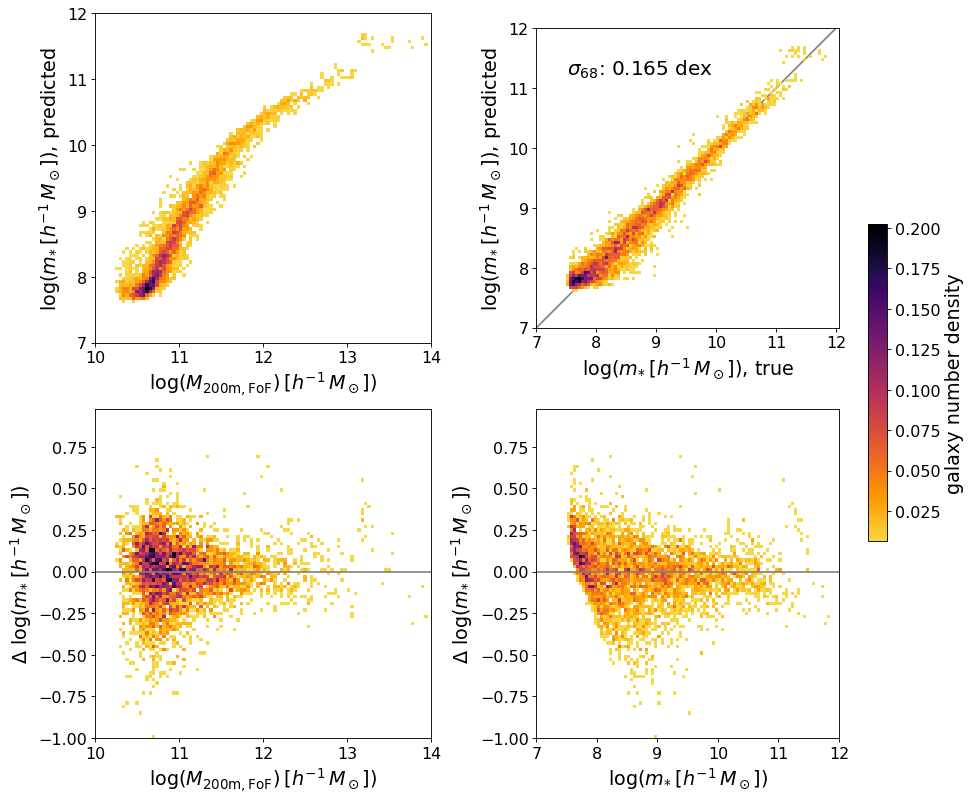
\includegraphics[width=0.7\columnwidth]{pred_mstellar.png}
    \caption{Predictions for the galaxy stellar mass $\mstellar$ using our invariant scalar features. The panels show the predicted stellar-to-halo mass relation, the predicted stellar mass compared to the true stellar mass, and the residuals of the stellar mass prediction compared to truth as a function of halo mass. The grey lines show zero error. The colorbar shows the number density of galaxies in units $(\hMpc)^{-3} \text{dex}^{-2}$, which takes into account the size of the box, the fraction of objects in the test sample, and the 2D histogram bin widths. We achieve accurate and precise predictions of the galaxy stellar mass with our invariant features.}
    \label{fig:mstellar}
\end{figure}

We focus on predicting the stellar mass of the central galaxy hosted by each DM halo, as this is the key quantity related to galaxy sample selection and is tightly correlated with other galaxy properties.
Our results with our fiducial feature set, the invariant scalar features with three radial bins, on our test sample of halos is shown in Figure~\ref{fig:mstellar}. 
In the top left we show the predicted stellar mass $\mstellar$ as a function of halo mass $\Mfof$; we see that we broadly recover the true shape of the stellar-to-halo mass relation. 
In the top right we show our predicted $\mstellar$ vs. the true $\mstellar$; our predictions are quite accurate, with a high density along the one-to-one line; the error $\sigma_{68}$, computed as the absolute symmetrized inner 68th percentile error, is 0.164 dex.

In the bottom row we show the absolute error (residuals) on our predictions as a function of halo mass and stellar mass.
We have larger errors at smaller halo and galaxy masses; this makes sense given the larger scatter in the stellar-to-halo mass relation at low halo masses, which is partially caused by shot noise dominating at those scales.
We also see an increase in error at high halo masses; this is related to the small sample size at those masses and the unbalanced training set in terms of halo size.
There is a clear artifact in the residuals as a function of stellar mass caused by our sample selection requirement that galaxies be composed of at least 50 star particles.
When the true stellar mass is very small, it is at the low edge of our training set and thus we are biased towards overpredicting it.
A practical tool could remedy this by using a wider training set than testing set to provide a buffer, or taking a multi-step approach to handle zero- and low-mass galaxies.  


\begin{figure}
    \centering
    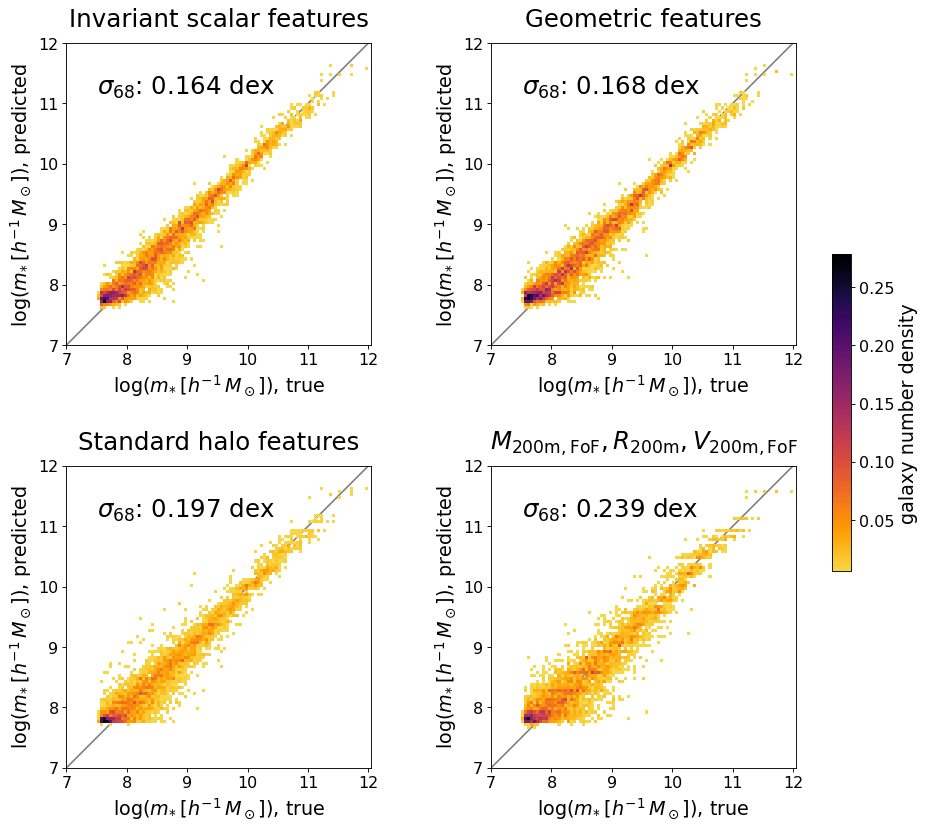
\includegraphics[width=0.7\columnwidth]{feature_comparison_mstellar.png}
    \caption{Predictions for the galaxy stellar mass based on different input feature sets: the invariant scalar features (our fiducial set); the components of the geometric features; a set of standard halo features; and only $\Mfof$, $\Rtwoh$, and $\Vfof$. These are detailed in \S\ref{sec:benchmarks}. The upper left panel is the same as the upper right panel in Figure~\ref{fig:mstellar}; the color bar is the same as in that figure as well. The invariant scalars approach outperforms the standard features in the stellar mass prediction, and significantly outperforms using only the mass and related scaling quantities. It very slightly outperforms the geometric feature set, which is not invariant to rotations.}
    \label{fig:mstellar_compare}
\end{figure}

We compare the performance our invariant scalars approach to other benchmark feature sets on galaxy stellar mass predictions in Figure~\ref{fig:mstellar_compare}.
Each panel shows the predicted vs. true stellar mass $\mstellar$ for a different feature set (detailed in \S\ref{sec:benchmarks}).
The invariant scalar features panel is reproduced from Figure~\ref{fig:mstellar}.
As expected, the worst-performing feature set is the one using only the basic global properties of the halo, $\Mfof$, $\Rtwoh$, and $\Vfof$ (recall that these are all directly related so this is essentially just a single scale), achieving just under a quarter of a dex in scatter.
We see some banding the predictions, likely due to the fact that this feature set can produce the mean stellar-to-halo mass relation but not the scatter.
The standard halo features, which includes the mass scale as well as a handful of shape and dynamical properties, performs better, with error reduced to under 0.2 dex. 

The geometric features produce still better predictions, suggesting that the detailed structure they encode---in both position and velocity space, and split into radial bins---adds significant information, giving an error 0.168 dex.
Somewhat surprisingly, we find that the invariant scalar features computed from these geometric features do not produce significantly improved predictions compared to the components of the geometric features.
The difference between these is that the geometric features are not invariant to rotations, while the scalar features are; both are invariant to translations, velocity boosts, and permutations, given how we construct the geometric features.
We expect that the invariance to rotations would become more important when using a smaller training set size, whereas the model seems able to learn the rotation invariance from our large and relatively homogenous training set.
It is also possible that the other symmetries are more dominant; in future work we could construct a benchmark that is not invariant to these symmetries for a clearer comparison.


\subsection{Predicting other baryonic properties}
\label{sec:pred_galprops}

\begin{figure}
    \centering
    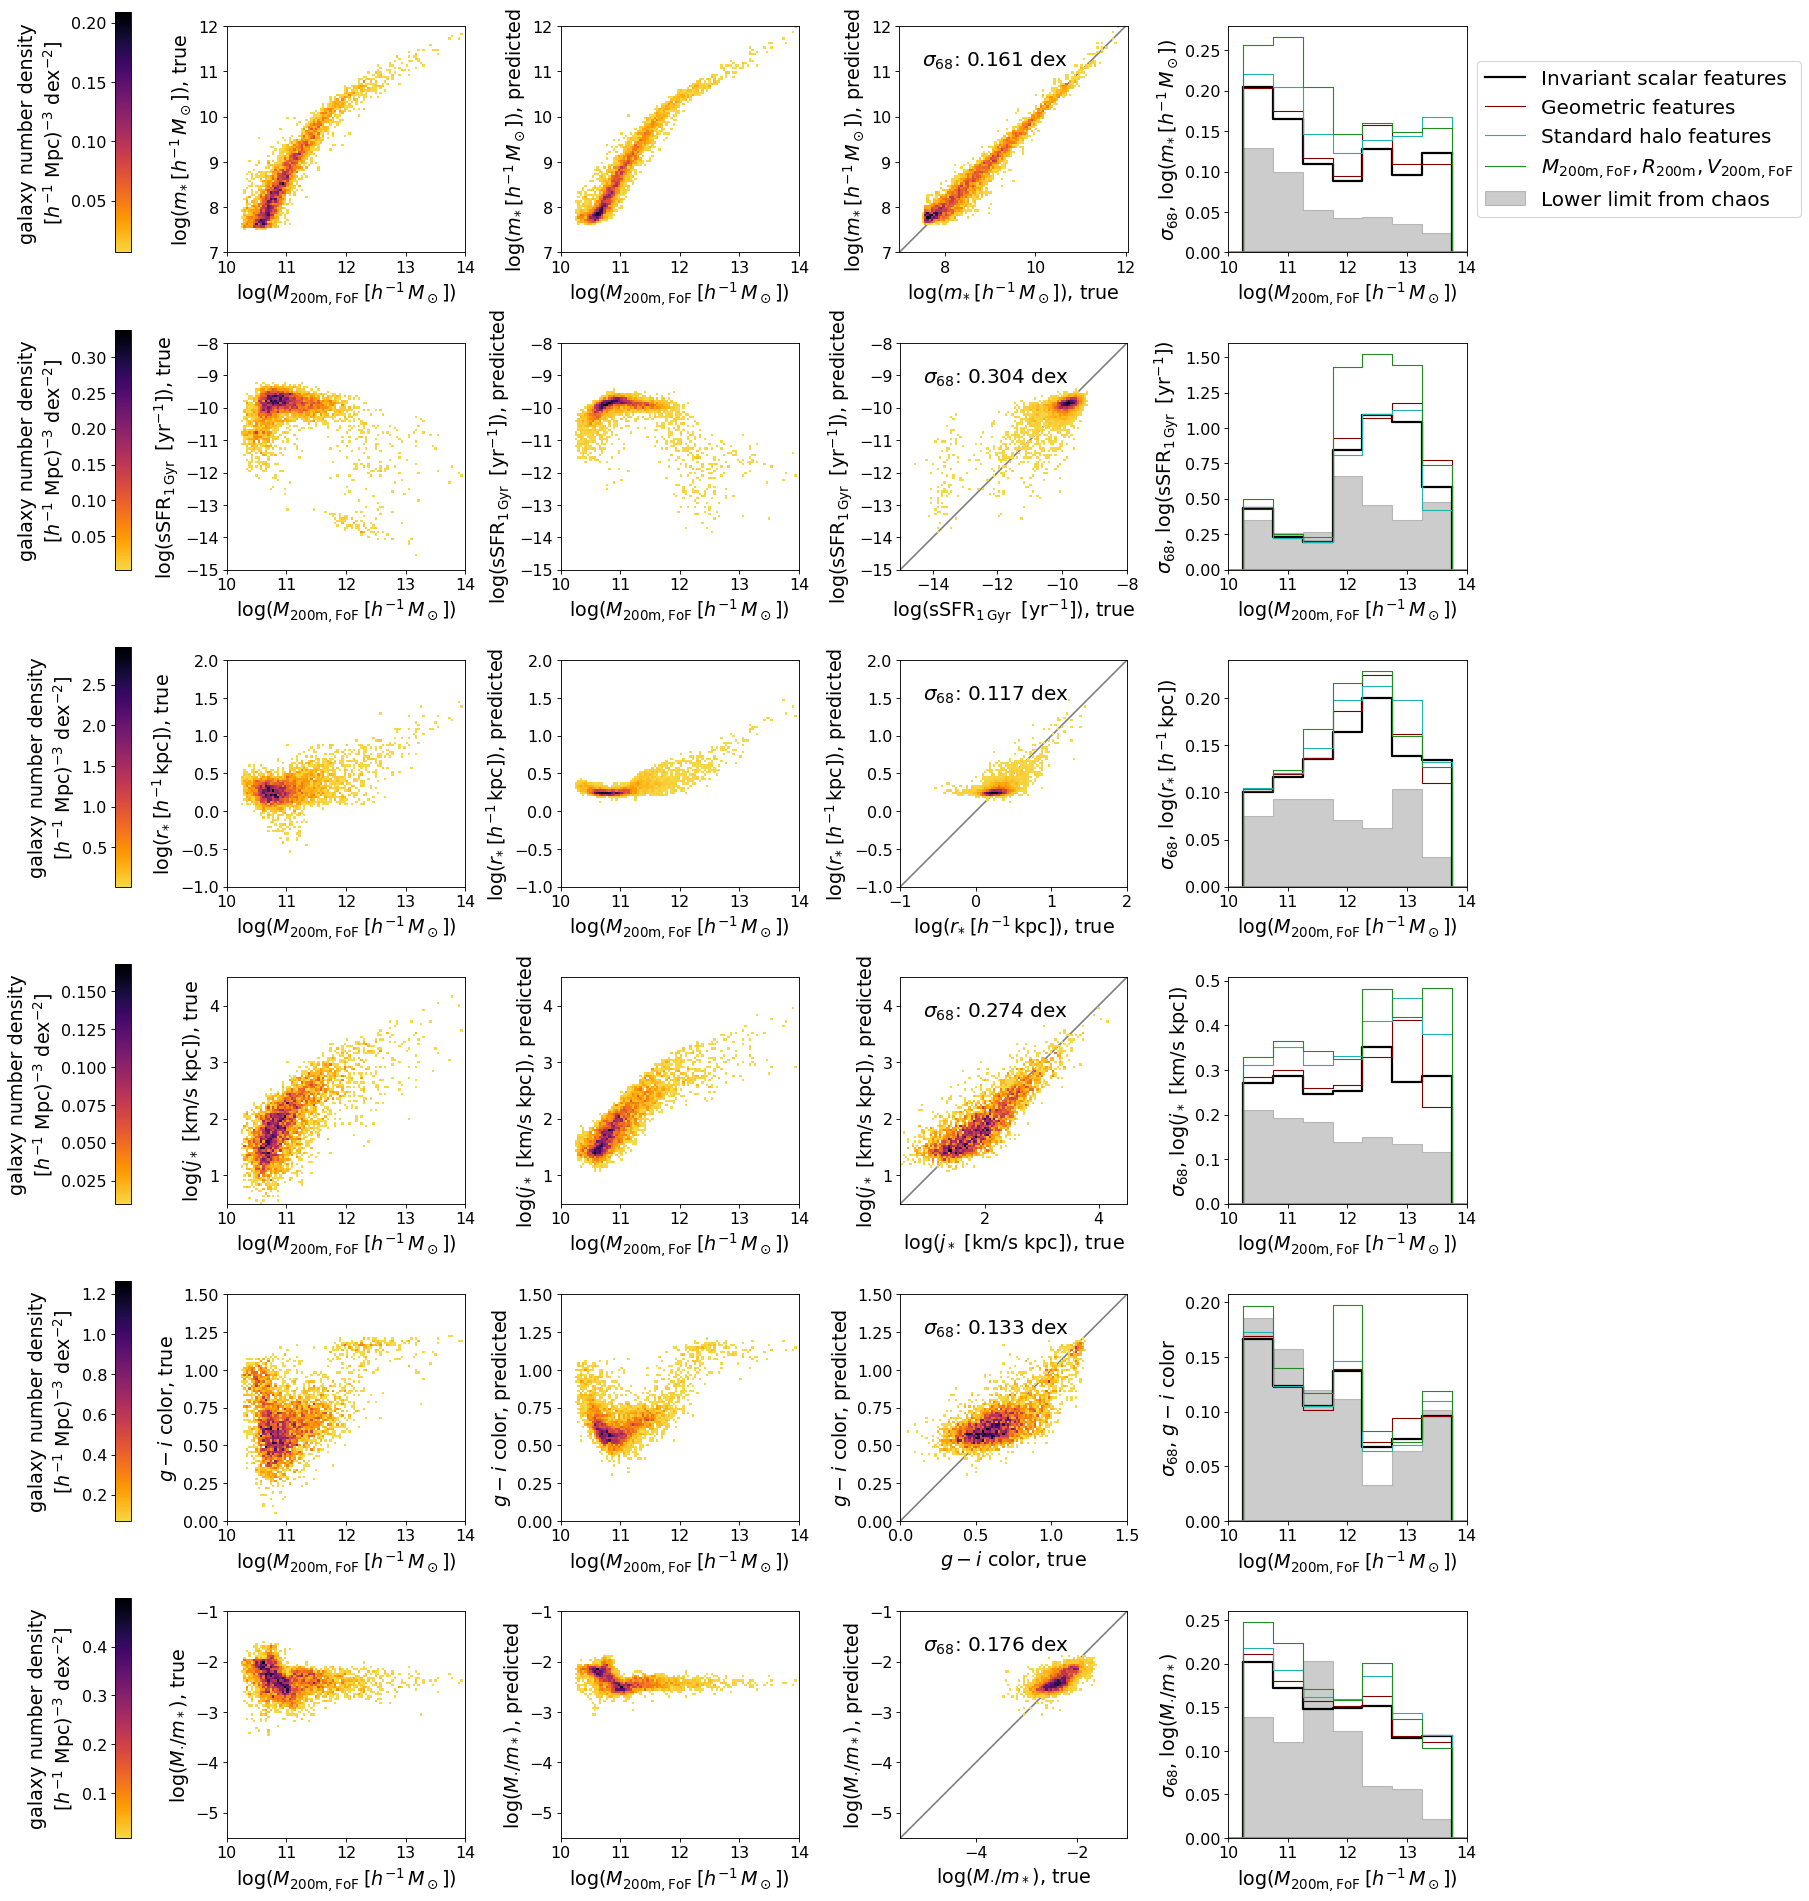
\includegraphics[width=0.8\columnwidth]{pred_galprops.png}
    \caption{Distributions and predictions of galaxy properties using our invariant scalars approach and other benchmark feature sets, for the test sample. 
    Each row shows a different galaxy property: stellar mass $\mstellar$, specific star formation rate $\ssfr$, stellar radius $\rstellar$, specific stellar angular momentum $\jstellar$, $\gminusi$ color, and black hole mass per stellar mass $\mbhpermstellar$. 
    The left column shows the property as a function of halo mass $\Mfof$. 
    The second column is the predicted distribution as a function of halo mass, and the third compared to the true property, using the fiducial invariant scalar features.
    The right is the binned error as a function of halo mass, comparing the scalar features (thick black), geometric feature components (red), standard features (blue), and mass scale features (green); the grey shaded region shows the lower limit from chaos.
    For most of the galaxy properties, the scalars slightly outperform the other features, but many properties are limited by chaos.
    }
    \label{fig:galprops}
\end{figure}

We show the results of our predictions on other galaxy and baryonic properties in Figure~\ref{fig:galprops}.
In the left two columns, we show the true and predicted distributions of properties as a function of halo mass $\Mfof$, where the predictions are with our fiducial invariant scalar features.
We see that we broadly reproduce the shape of the distribution for all of the properties. 
However, there are significant differences; noteably, nearly all of our predictions fail to reproduce the full scatter of the true distributions, tending towards the mean.
Generally, the regions of poor prediction indicate that either our features are not informative enough, our model is not performant enough, or there is a fundamental limitation in the amount of information accessible---or some combination of these three.

We investigate the final possibility by comparing the error in our results to the scatter from chaos, as computed from the ``butterfly'' simulations of \cite{Genel2019} (described in \S\ref{sec:galprops}), which represents a limit to the retrievable information.
This is shown as a function of halo mass in the grey shaded region in the final column, compared to the binned error of our predictions.
We see that for some properties in some regimes, we are indeed at or near the chaotic limit, where we expect the rest of the information is destroyed by the chaotic effects of evolution.
This is the case for the $\ssfr$ and $\rstellar$ at low halo masses, for $\gminusi$ color at all masses, and $\mbhpermstellar$ at intermediate masses.
For these cases, we are able to reproduce the relatively complex shape of the property distribution as a function of halo mass: for instance for the $\ssfr$ we accurately predict the sharp transition from large scatter at very low halo mass to low scatter at intermediate halo mass, and for $\gminusi$ color we predict the non-monotonic shape of the distribution vs. halo mass, including the large colors of the high-mass galaxy population.
In some bins we are achieving results below the chaotic limit; this may be because this is a somewhat optimistic limit as it is computed from a slightly higher resolution simulation, and also possibly due to small number statistics (generally for the butterfly simulations, and especially for the high mass bins in both).

There are some populations that our predictions fail to reproduce, somewhat separate from the low-scatter issue.
For instance, we do not predict the very low $\rstellar$ ``fin'' at low halo masses, leading to consistent over-predictions in that bin.
Our model also struggles to handle very low values, such as in the $\ssfr$ distribution where we replaced the value of galaxies with no star formation with a small limit, as can be seen in the intermediate-to-high mass regime (where galaxies are more likely to be quenched).
We see that our predictions do not separate out this population, instead predicting a continuous distribution of specific star formation rates at those masses.
While some of our predictions of baryonic properties are impressive and show that there is significant information in halo shape relevant to galaxy properties, our results broadly align with other recent findings that baryonic properties beyond stellar mass are difficult to predict using halo features \citep{de_santi_mimicking_2021,stiskalek_scatter_2022}.

In the right column of Figure~\ref{fig:galprops}, we show the comparison between our invariant scalars approach with the other benchmark feature sets.
We find that while the scalars generally outperform the other features, the differences are not particular pronounced for most properties and scales.
The clearest improvements of the scalars over the standard features are seen in predicting the stellar mass $\mstellar$, as discussed in \S\ref{sec:pred_mstellar}, and the specific stellar angular momentum $\jstellar$; the latter may be thanks to our inclusion of high-order velocity-space features, while the standard features only use the velocity dispersion and spin.
Similarly to the stellar mass case, we do not see a clear difference between predictions with the scalar features and geometric features, indicating that the model is able to learn the rotational invariance from the data even when the features are not invariant.


\subsection{The mass assembly history encoded in the present-day halo shape}


\begin{figure}
    \centering
    \includegraphics[width=0.5\columnwidth]{pred_mah.png}
    \caption{The predicted mass assembly history of a halo based on the invariant shape scalars. The top panel shows the MAHs of a random selection of halos from the test set, and the predicted scale factor at each mass fraction. The middle panel shows the fractional residuals between the two, and the bottom shows the inner 68th percentile of the predictions for all of our test set, compared to that of the distribution of MAHs used in training. \ksf{rn im plotting test set for latter, make sure to switch to test!}}
    \label{fig:mah}
\end{figure}


\subsection{Understanding the relative importance of the halo shape features}

The feature subsets we consider are: only mass features; mass and position features; mass and velocity features; mass, position and velocity features.
We also investigate limiting to certain orders in $O(x)+O(v)$: 0, 2, and 4.
Finally, we consider different numbers of bins, as well as excluding cross-bins.

\begin{figure}
    \centering
    %\includegraphics{}
    \caption{The precision on the predictions of the given property when using the denoted subset of invariant scalars.}
    \label{fig:features}
\end{figure}


\section{Discussion}
\label{sec:discussion}

Topics/points for discussion section:
\begin{itemize}
    \item Understanding of important features (what do they mean, relationship to currently used features)
    \item Application of approach to useful tasks (constructing mock catalogs, predicting galaxy properties in larger \& higher res simulations and being able to construct many realizations)
    \item The inference problem: going from galaxies to DM
    \item Feature construction choices (e.g. could construct geometric features other ways like with spherical harmonics)
    \item Future goal to move away from halo framework and work on full particle distribution, starting from e.g. density peaks. Intermediate task is to start from halo centers but include all particles, not just those in FoF group
    \item Future work to look at impact of larger-scale environment, incorporate it in input features
    \item Other properties we should predict (position: discuss offsets bw dark and hydro; spin: pseudo-vector)
    \item particles have large time derivative; galaxy has relatively small time derivative! we could show this with our scalars. discuss time dependence.
\end{itemize}


\section{Chapter Acknowledgements}
The authors would like to acknowledge very helpful discussions with Soichiro Hattori, Austen Gabrielpillai, Ben Blum-Smith, Weichi Yao, Scott Tremaine, Rachel Somerville, Derek Lim, and Benjamin Wandelt.
The authors also thank useful feedback by participants of the Flatiron CCA Astrodata Group, Galaxy Formation Group, and Cosmology X Data Science Group.
This research was performed in part at the Coworking Retreat on Equivariant Machine Learning held at the Johns Hopkins University in March 2023.
K.S.F.~is supported by the NASA FINESST program under award number 80NSSC20K1545.
This research made use of computational resources at New York University; we thank the NYU high-performance computing team.